\section{INTRODUCTION}

As a research university, we offer undergraduate students opportunities to work on major research projects, with different students rotating in and out, semester to semester. For those more interested in the applied disciplines (e.g. engineering, journalism, law, business, social work) there are fewer such opportunities. Our innovation is a course design which would give the “major project” experience in an experiential form, for students in the applied disciplines. We call it multi-semester/multi-cohort. 

\begin{figure}[!h]
  \centering
  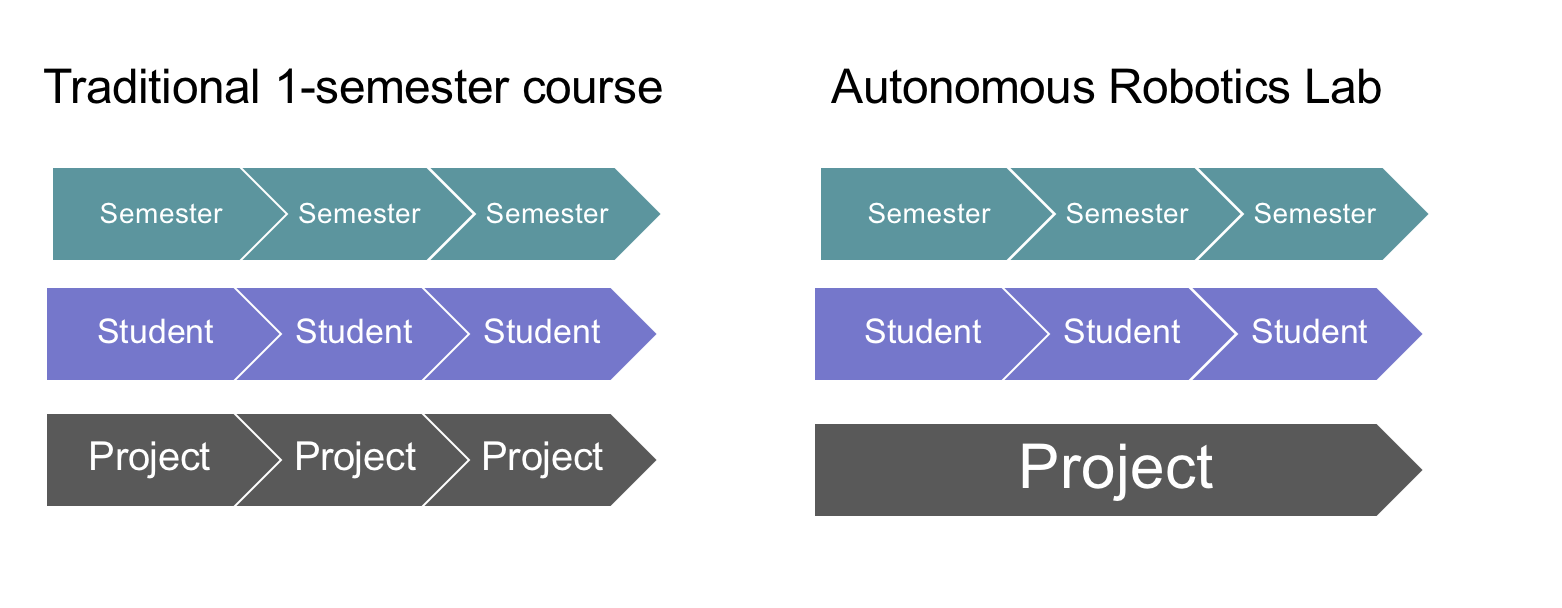
\includegraphics[width=\columnwidth,height=6cm]{diag1}
  \caption{Multi Semester/Multi Cohort structure}
  \label{fig:diag1}
\end{figure}

``Multi-semester" because the project will not (cannot) be completed in one semester, and “multi-cohort” because the set of students working on it changes from semester to semester. We wanted to see whether it would work, and learn how to organize things to allow each semester’s cohort to pass knowledge to the next one in an efficient way, and how assessment would work.


We are inspired by the idea of a “BHAG” (Big Hairy Audacious Goal), conceptualized in \cite{Collins}. Collins and Porras describe this mouthful term as follows:

\begin{quote}
``We found in our research that visionary companies often use bold missions – [BHAGs,shorthand for Big, Hairy, Audacious Goals] - as a powerful way to stimulate progress. [All companies have goals...] A true BHAG is clear and compelling, serves as a unifying focal point of effort, and acts as a catalyst for team spirit. It has a clear finish line, so the organization can know when it has achieved the [goal] A BHAG engages people – it reaches out and grabs them. It is tangible, energizing, highly focused.``\cite{Collins}
\end{quote}

For our course, our BHAG is "Campus Rover", a robot that can travel both indoors and outdoors on campus to deliver packages from an office in one building to an office in another building.After our first semester pilot, we made changes and refinements in the program, and we are now in our second semester. This paper describes the curriculum and how it has evolved, and explores what works and does not.

\section{The Course}

We call our course “Autonomous Robotics Lab”. It is offered every semester, initially to a maximum of 12 students. As mentioned, in order to provide continuity and a sense of a greater purpose, we choose a “major project” objective which was compelling to students, could not be solved in one semester, and provided the kind of learning opportunities that we were after. 

The goal we set for ourselves is the creation of an autonomously navigating robot that could pick up and deliver small packages across campus. As it turns out this is in general an unsolved problem with plenty of juicy subproblems to keep us occupied indefinitely.

\subsection{Who is admitted} As an experimental course we are being highly selective of the (up to 12) students who can take this course, to allow us some margin of error in organizing and structuring the course. We are admitting only Juniors, Seniors and Graduate students. We administer this as follows: The catalog lists the course as requiring permission from the instructor. When students respond they are asked to fill out a short (Google) survey asking about grades received in key Computer Science courses as well as a statement of qualification stating in their own words what previous experiences prepare them for the course. And finally, they are individually interviewed over email to determine that they are strong programmers, disciplined, motivated and with a demonstrated track record.

\subsection{Project and team-based learning} Given that each semester would be different we had to have a clear sense of our learning objectives. In a general sense, the goal is to expose students to the problem solving learning that comes into play when working on a large software project with many moving parts.

\subsection{Learning Objectives} Our objectives fall into two categoies, Robotics and Software Engineering. Here they are, edited for length:

\begin{itemize}
\item Demonstrate understanding of how a simple wheeled robot works, how to control it through software, learning some key algorithms along the way, and implementing the code for a series of more and complicated challenges.
\item Demonstrate the ability to design, implement and test programs written for ROS (Robot Operating System.) Demonstrate understanding of the key concepts of ROS, nodes, topics, commands and services.
\item Be effective working in teams, designing new algorithms and solving problems of navigation and robotics, brainstorming, collaborating, implementing, testing and demonstrating the results of their work.
\item Demonstrate professional and agile software engineering processes, including writing elegant, readable, documented code, working in rapid iterations, each with a goal and a demo, and performing weekly standup meetings.
\end{itemize}

\section{Review of Relevant Literature}

There does not appear to be an established literature on what we have called a ``Multi Semester/Multi'' Disciplinary” Course design. At least we have not been able to pin one down, neither in Engineering or other disciplines. That is not to say that our approach is unique, or never been tried before, but more that it appears that the terminology and conceptual frameworks have not coalesced in a discernible way. 

For example, in “Learning by Doing: Reflections of the Epics Program \cite{Epics}, Zoltowski and Oakes describe a “multidisciplinary, vertically-integrated, student led, service-learning design course”, where students of all levels join and participate in multi-semester service projects built around a central framework, called “Epics”. 

“However, in EPICS, the time lines are decoupled, so that projects can extend beyond one academic term. This allows us to scope projects to meet the needs of the community partner, not the requirements of the academic time line. It allows for iteration within the design process as problems and improvements are identified. In addition, students can participate in multiple semesters.”

An interesting feature is that the courses count for one half the normal course credits, which allows students to take the course more than once. This could be used to help create continuity from semester to semester, as will be described below.

\section{Challenges}

\subsection{Technology} Robotics is an interesting discipline in that it is equal parts software and hardware, and equal parts theory and practice. Over two semesters so far, we’ve honed in on a software platform (“ROS” \cite{ROS}) and a hardware platform (“Turtlebot” \cite{Turtle}) that have the right characteristics needed as of now. These are both highly complex, and while appropriate, present a major learning curve for the students.

\subsection{Curriculum Design} The curriculum is built around the long term goal of the “Campus Rover” (see above) and while students aren’t actually implementing that yet, it gives form and meaning to the curriculum. To support the intended learning objectives, the majority of the time is allotted to students work in teams. 

Each semester could have different team "sub" missions, depending on the size of the group, their interests and abilities, and the status of the project. In the current semester, for example, the teams are: “Architecture”, “Navigation” and “New Platform”.

\subsection{Continuity}A major challenge is built in to the “multi-cohort’ structure. Each semester there are a brand new group of students! From the very beginning, during the “recruiting” process, we emphasize the importance of continuity, of leaving the table “set” for the next group coming next semester. We are exploring many possible ways of doing this, some we have implemented:
\subsubsection{Documentation}During the semester, and especially during the last week, students are charged with documenting their achievements (and non-achievements), including software, procedures, videos, check-lists, open issues, etc. 
\subsubsection{Teaching Assistant}We try to recruit next semester’s teaching assistant from among this semester’s cohort. Because we choose top students, the majority of them are Seniors or grad students who will not be around in the coming semester. With funding, we are considering having a part-time, but year-round grad student staff to help provide the continuity.
\subsubsection{Lab Notebooks}Students were asked to maintain an online "Lab Notebook" with the expectation and intent that these would be useful both for assessment and for continuity. In practice, this did not work very well, as it was difficult to motivate students to maintain their notebooks, and in the end they were chaotic and hard to reuse.

\subsection{Assessment} Given the highly ambitious and even speculative nature of the main project, we do not assess on “success of the project”, that is, whether students succeeded in building the Campus Rover. Rather, our assessments look at:

\subsubsection{Participation}Because the course relies on students’ ability to self-manage and self-organize. Students have to demonstrate their ability make progress without the professor or the curriculum dictating the exact steps they need to take. Participation therefore is more than just showing up for the weekly 3 hour meeting. It means showing up for your teammates as well. In discussions it is apparent that students really appreciate this freedom and responsibility - although not every student is ready for it.

\subsubsection{Demonstrations}As mentioned, each week (after the first 3) teams need to put in writing what they will focus on for the coming week and what they will demonstrate during the following week. Students have to learn and then be motivated to think in terms of concrete weekly objectives, followed by a demonstration to the rest of the class. We track this during the semester.

\subsubsection{Content}As mentioned, at the end of the semester we ask that the results of the work of each team be documented. We provide a general idea of what forms the documentation might take, but it is up to the students to digest the results of the semester and write them up in a way that makes sense to the next cohort.


\section{Progress to date}
As we enter the third semester of this program, we judge it a qualified success. In this final section we will review key features of the course design and our view of how well they worked, and suggestions for others meaning to implement a Multi-semester/Multi-cohort curriculum.
\subsection{What worked}
\begin{itemize}
\item BHAG: We feel that a having a overarching goal (BHAG) to frame the whole experience is very important. The characteristics we would look for are:
\begin{itemize}
\item A project which inspires and excites
\item A project which one can imagine is very hard, but not impossible
\item A project that students will want to talk about to friends and family
\end{itemize}

\item Robotics: Our students have demonstrated learning of advanced Robotics and Software Engineering concepts and skills. However as you see below, this learning did take valuable time out of the semester. Ideally there would be a preparatory course that would be a required pre-requisite.
\item Recruiting: While somewhat time consuming, our view is that it is essential to hand pick students. For us, requiring Juniors or above (although we have made exceptions) is a good starting point. However in addition we look for students who show great motivation, and history of persistence and inventiveness. We also give a frank preview of the likely challenges that they will encounter.
\item Lab: We have found that the lab “dynamic” is positive and energetic. Interestingly the cohort in one semester has shown a sense of obligation to those coming the next semester. We think this is a consequence of framing the individual semester within the context of the large overarching goal.
\item Outreach: We have been able to use the course as a platform for building and extending contacts with the robotics industry.
\item Team model: Dividing up the students into teams is important. And it is important to design team-objectives which are:
  \begin{itemize}
  \item Clearly supportive of the overarching goal (BHAG)
  \item Suitable for a team of approximately 3 students
  \item Self-contained so that the team can organize their own work and understand what their objectives are.
  \end{itemize}
Choosing the team objectives is the role of the instructor with input from the students. It is important to be able to explain to the students exactly what the team objective is, what it means, how it fits in the big picture, and suggestions on how it may be tackled. With that, the students are allowed organize themselves based on their interests and abilities.
\end{itemize}

\subsection{What we are still working on}
\begin{itemize}
\item Learning Curve: Learning the fundamentals of robotics (software and hardware) represents a very steep learning curve which means that we are not getting into the actual projects until 1/4 to 1/3 into the semester
\item Semester Deliverables: Until we achieve our BHAG, we need to figure out more satisfying “Semester Completion Deliverables” at the end of each semester.

\item Lab Notebook: As mentioned earlier, a feature of the course is the requirement that each student keep a ``lab notebook'' that they update with their progress, successes and setbacks, and notes to refer to later in the semester. Our idea was that this would serve as an assessment tool. This has not worked out. It was never updated, and when it was updated it felt like a ``make-work'' chore. However it has morphed into a true Lab Notebook, used, not for assessment, but as a way to help the student and student teams keep notes that they would use in future weeks.
\end{itemize}
\section{Some next steps and conclusion}

\begin{itemize}
\item The course will continue to evolve, and will run at least two more semesters so we can feel like we conducted a thorough trial.
\item We are about to study other disciplines who have built courses in an analogous way, to compare lessons learned, what worked well and what could be improved. Our current prospective targets are Architecture and Environmental Studies.
\end{itemize}

We are very encouraged by our progress to date in piloting this approach to teaching robotics. The course has run for two semesters and will run at least two times more in the coming year. We expect to have a more detailed report at that point.

